% Annexes techniques du dossier professionnel.
% Les lettres B et D sont volontairement conservées pour correspondre aux
% documents déjà préparés et numérotés ainsi dans leur contenu.
% Chaque annexe possède un label stable afin que les renvois du corps du
% dossier restent valides lorsque de nouvelles annexes sont ajoutées.

\chapter{Proposition d'architecture initiale pour le flux FCU}
\label{ann:fcu-architecture}

Cette proposition d'architecture correspond à une étape de conception du projet FCU. Elle est conservée comme trace de la démarche et des arbitrages ayant conduit à la solution finalement mise en production.


\includepdf[
  pages=-,
  pagecommand={\thispagestyle{plain}}
]{figures/annexes/proposition_architecture_FCU.pdf}

\chapter{Diagramme détaillé de la chaîne Ediacara}
\label{ann:ediacara-diagramme}

Le document suivant reproduit le diagramme détaillé utilisé pour rétro-documenter la chaîne Ediacara. Sa taille justifie son placement en annexe plutôt que dans le corps du chapitre consacré au projet FCU / Ediacara.

\includepdf[
  pages=-,
  pagecommand={\thispagestyle{plain}}
]{figures/annexes/Annexe_B_Ediacara_decoupee.pdf}

\chapter{Procédure de mise en production d'Ediacara}
\label{ann:fcu-mep}

La procédure suivante constitue le guide opérationnel préparé pour sécuriser l'intervention sur l'environnement de production, documenter les modifications à réaliser et permettre un retour arrière contrôlé.


\includepdf[
  pages=-,
  pagecommand={\thispagestyle{plain}}
]{figures/annexes/mise_en_prod_ediacara.pdf}

\chapter{Diagramme complet du modèle S-100 / S-123}
\label{ann:s123-modele}

Le document suivant reproduit le diagramme complet du modèle étudié dans le projet S-123. Le chapitre principal conserve une représentation simplifiée ; cette annexe permet d'examiner la structure détaillée.

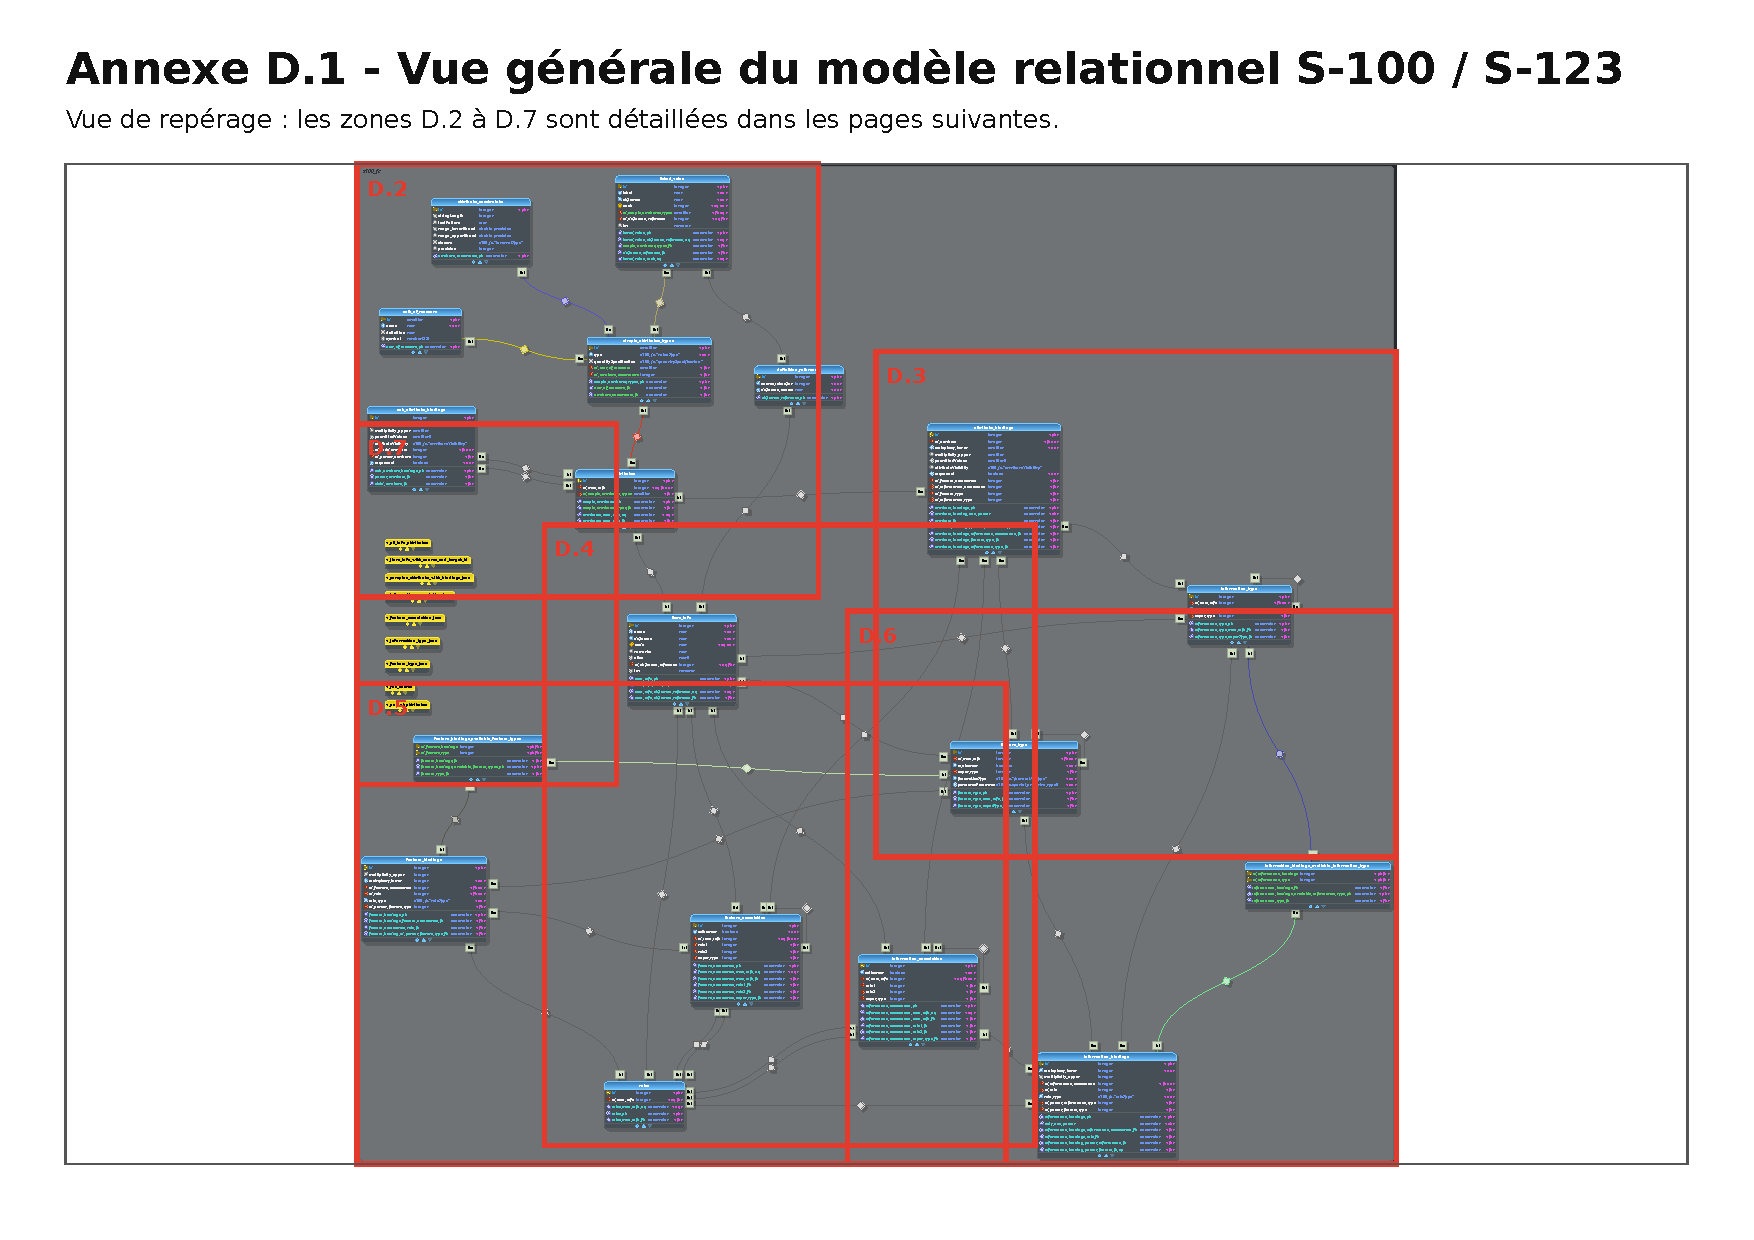
\includepdf[
  pages=-,
  pagecommand={\thispagestyle{plain}}
]{figures/annexes/Annexe_D_S100_S123_decoupee.pdf}

\chapter{Extraits de la documentation MkDocs d'Ediacara}
\label{ann:ediacara-mkdocs}

Les vues suivantes illustrent la documentation produite pour capitaliser la compréhension de la chaîne et faciliter sa maintenance par l'équipe.

\begin{figure}[H]
  \centering
  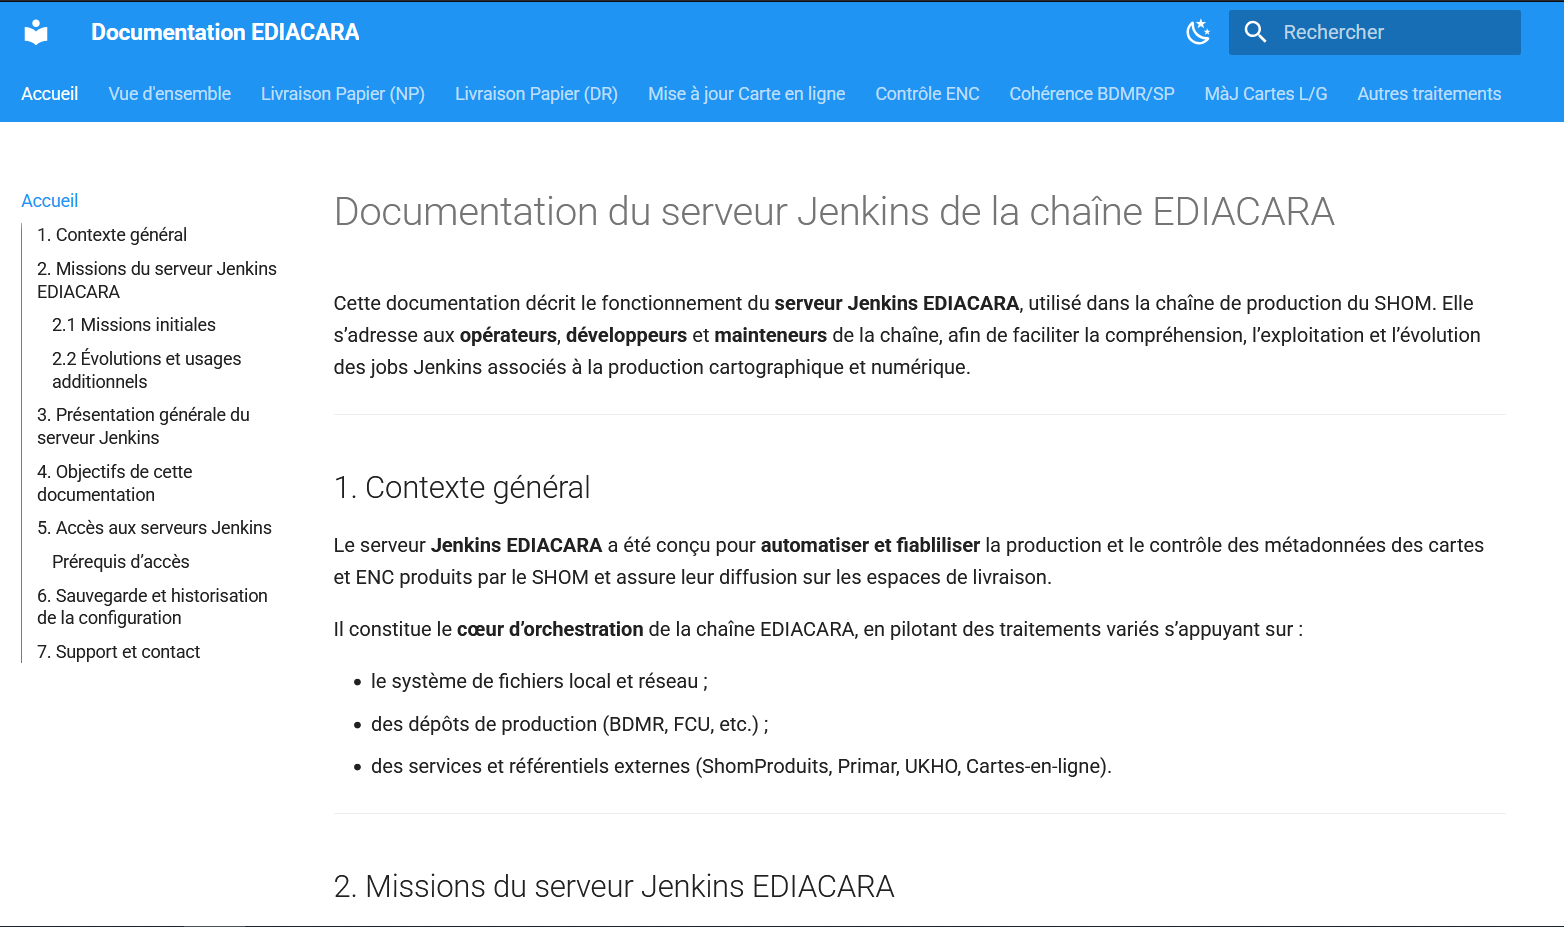
\includegraphics[width=\textwidth,height=0.72\textheight,keepaspectratio]{figures/annexes/acceuil_doc_mkdocs.PNG}
  \caption{Page d'accueil de la documentation MkDocs d'Ediacara}
  \label{fig:ann-mkdocs-accueil}
\end{figure}

\begin{figure}[H]
  \centering
  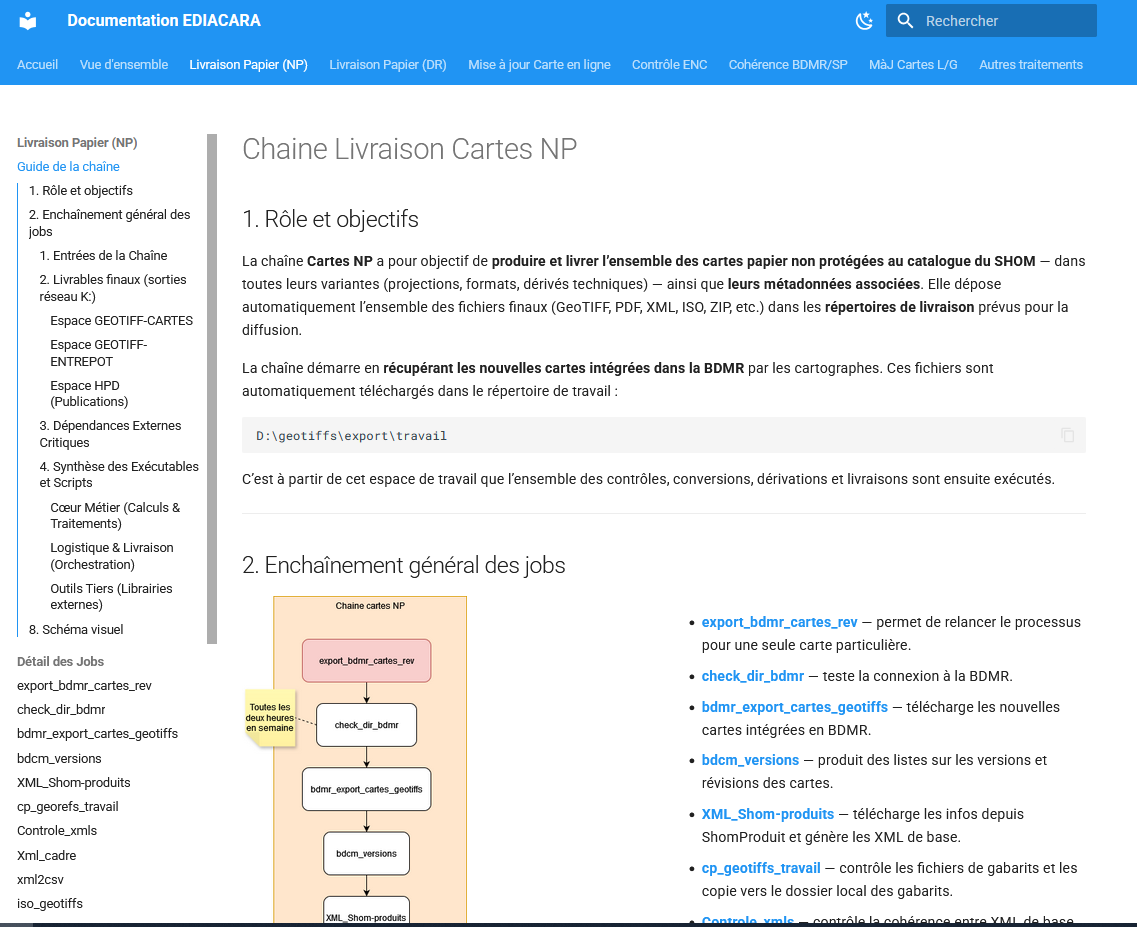
\includegraphics[width=\textwidth,height=0.72\textheight,keepaspectratio]{figures/annexes/acceuil_chaine_np_mkdocs.PNG}
  \caption{Présentation de la chaîne NP dans la documentation MkDocs}
  \label{fig:ann-mkdocs-np}
\end{figure}

\chapter{Exemple de job de contrôle GeoTIFF dans Ediacara}
\label{ann:ediacara-geotiff}

Les captures suivantes présentent un exemple représentatif de job Jenkins de contrôle GeoTIFF. Elles complètent la description de la chaîne sans imposer au lecteur des captures de configuration détaillées dans le corps du dossier.

\begin{figure}[H]
  \centering
  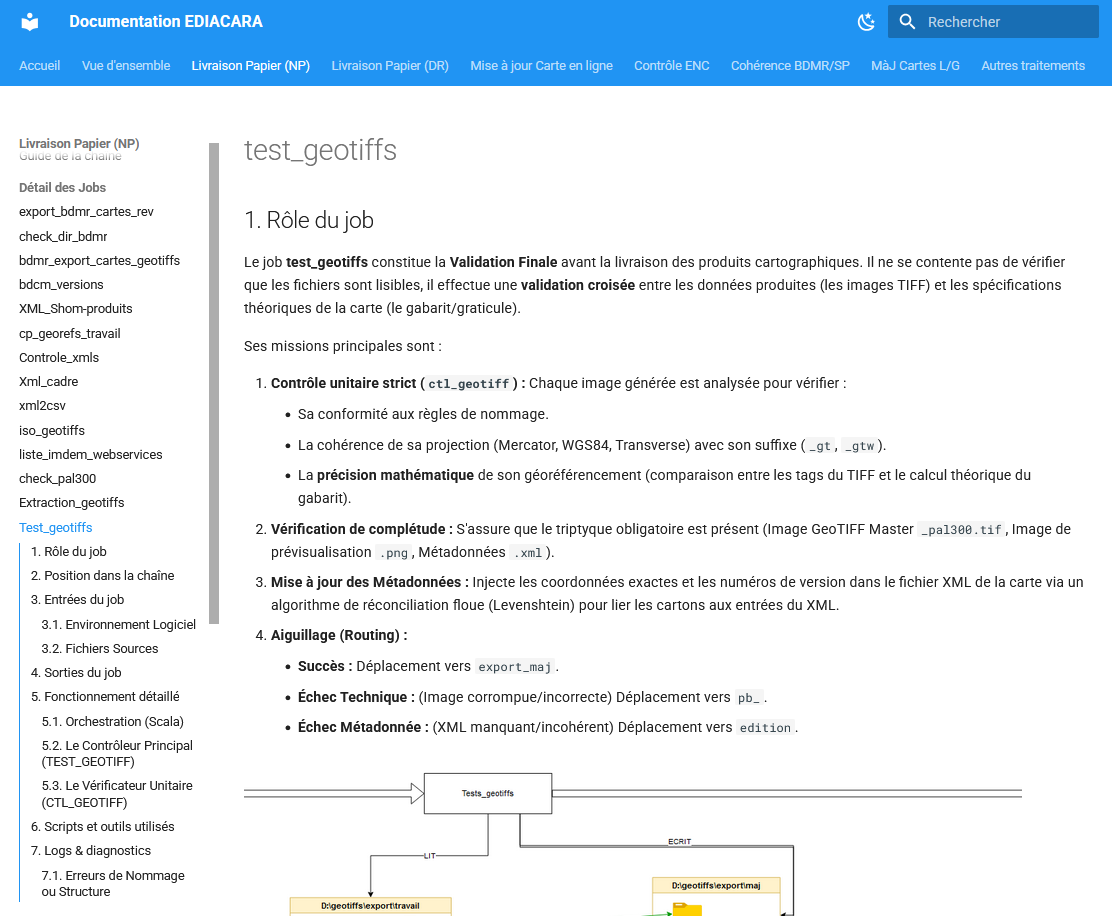
\includegraphics[width=\textwidth,height=0.72\textheight,keepaspectratio]{figures/annexes/exemple_job_test_geotiffs_1.PNG}
  \caption{Exemple de job de contrôle GeoTIFF -- vue 1}
\end{figure}

\begin{figure}[H]
  \centering
  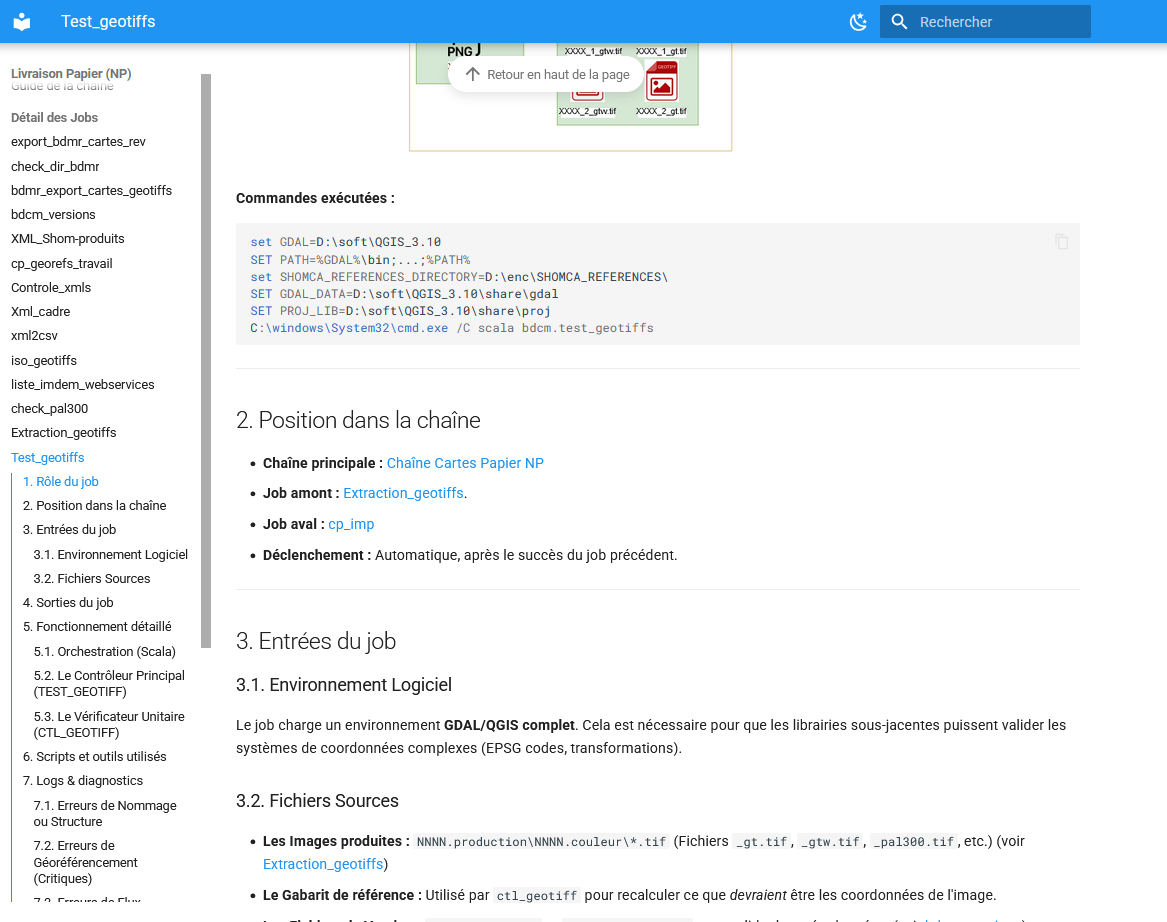
\includegraphics[width=\textwidth,height=0.72\textheight,keepaspectratio]{figures/annexes/exemple_job_test_geotiffs_2.PNG}
  \caption{Exemple de job de contrôle GeoTIFF -- vue 2}
\end{figure}

\begin{figure}[H]
  \centering
  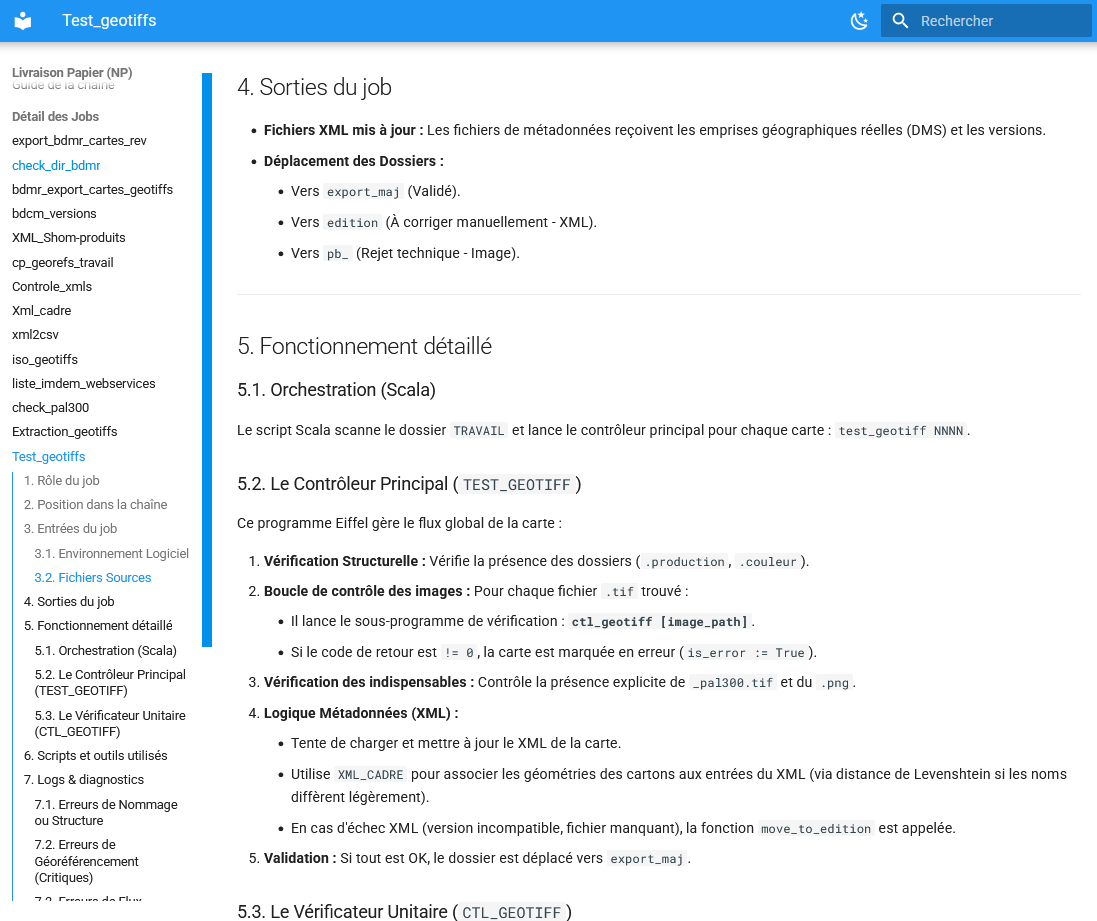
\includegraphics[width=\textwidth,height=0.72\textheight,keepaspectratio]{figures/annexes/exemple_job_test_geotiffs_3.PNG}
  \caption{Exemple de job de contrôle GeoTIFF -- vue 3}
\end{figure}

\chapter{Pipeline CI et tests du projet piv2glz}
\label{ann:piv2glz-ci}

Ces captures constituent des preuves complémentaires de l'automatisation décrite dans le chapitre \texttt{piv2glz} : pipeline GitLab CI/CD, configuration de la CI et extrait de la suite de tests.

\begin{figure}[H]
  \centering
  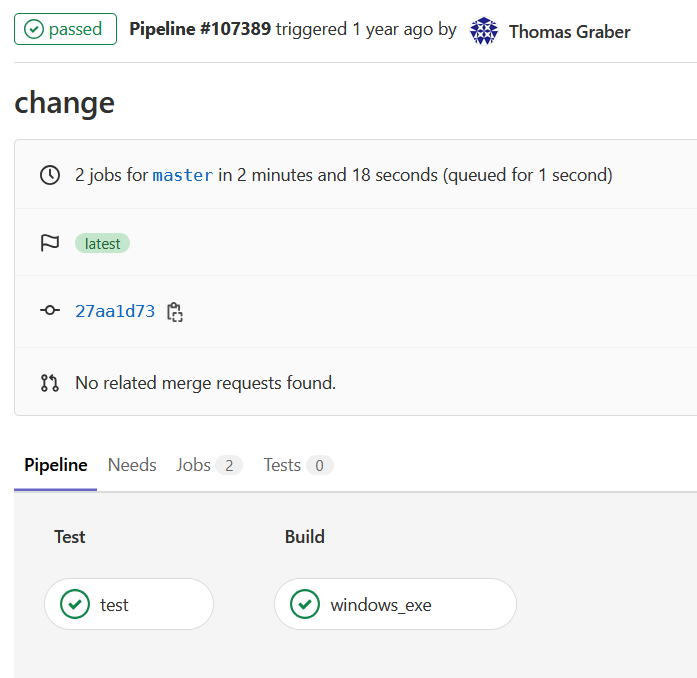
\includegraphics[width=\textwidth,height=0.72\textheight,keepaspectratio]{figures/annexes/pipeline_ci_cd_piv2glz.PNG}
  \caption{Pipeline CI/CD du projet piv2glz}
  \label{fig:ann-piv2glz-pipeline}
\end{figure}

\begin{figure}[H]
  \centering
  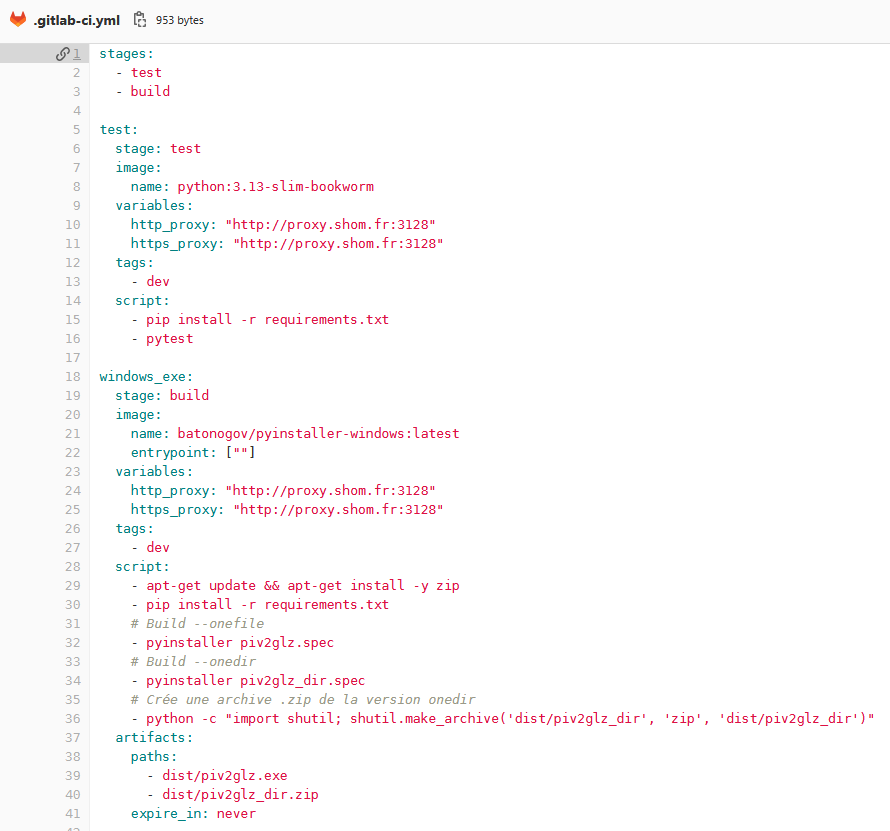
\includegraphics[width=\textwidth,height=0.72\textheight,keepaspectratio]{figures/annexes/code_ci_piv2glz.PNG}
  \caption{Extrait de la configuration CI de piv2glz}
  \label{fig:ann-piv2glz-code-ci}
\end{figure}

\begin{figure}[H]
  \centering
  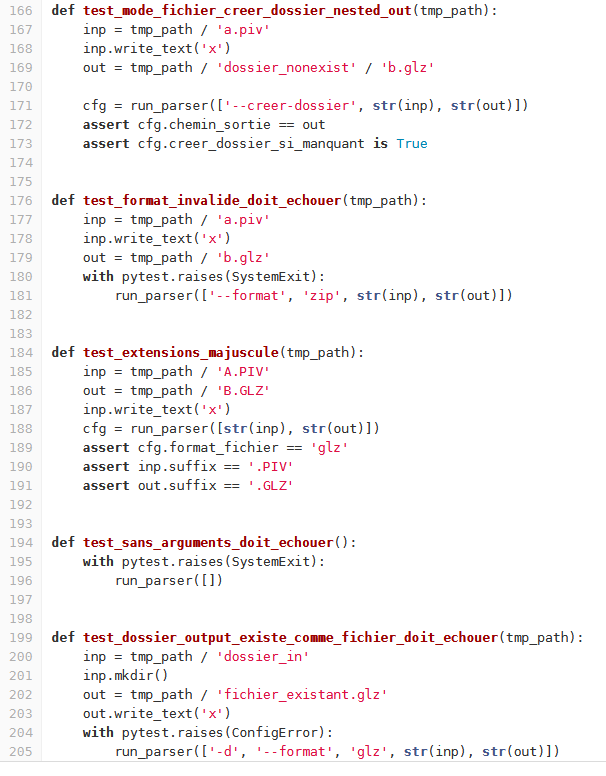
\includegraphics[width=\textwidth,height=0.72\textheight,keepaspectratio]{figures/annexes/extrait_code_test_piv2glz.PNG}
  \caption{Extrait de la suite de tests de piv2glz}
  \label{fig:ann-piv2glz-tests}
\end{figure}
